\documentclass{beamer}
\beamertemplatenavigationsymbolsempty
\usecolortheme{beaver}
\setbeamertemplate{blocks}[rounded=true, shadow=true]
\setbeamertemplate{footline}[page number]
%
\usepackage[utf8]{inputenc}
\usepackage[english,russian]{babel}
\usepackage{amssymb,amsfonts,amsmath,mathtext}
\usepackage{subfig}
\usepackage[all]{xy} % xy package for diagrams
\usepackage{array}
\usepackage{multicol}% many columns in slide
\usepackage{hyperref}% urls
\usepackage{hhline}%tables
% Your figures are here:
\graphicspath{ {fig/} {../figures/} }
\usepackage{algorithm}
\usepackage{algpseudocode}

%----------------------------------------------------------------------------------------------------------
\title[\hbox to 56mm{Neural SDE}]{Neural SDE для нахождения моментов разладки временных рядов}
\author[И.\,Д. Папай]{Папай Иван Дмитриевич}
\institute{Московский физико-технический институт}
\date{\footnotesize
\par\smallskip\emph{Курс:} Автоматизация научных исследований\par (практика, В.\,В.~Стрижов)/Группа 128б
\par\smallskip\emph{Эксперт:} В.\,В.~Стрижов
\par\smallskip\emph{Консультант:} Э.\,А.~Владимиров
\par\bigskip\small 2024}
%----------------------------------------------------------------------------------------------------------
\begin{document}
%----------------------------------------------------------------------------------------------------------
\begin{frame}
\thispagestyle{empty}
\maketitle
\end{frame}
%-----------------------------------------------------------------------------------------------------
% \begin{frame}{Цель исследования}
%\begin{block}{Решается задача}
%\end{block}
% \end{frame}
%-----------------------------------------------------------------------------------------------------
\begin{frame}{Предмет исследования}

\begin{columns}[c]
\column{0.5\textwidth}
\begin{figure}
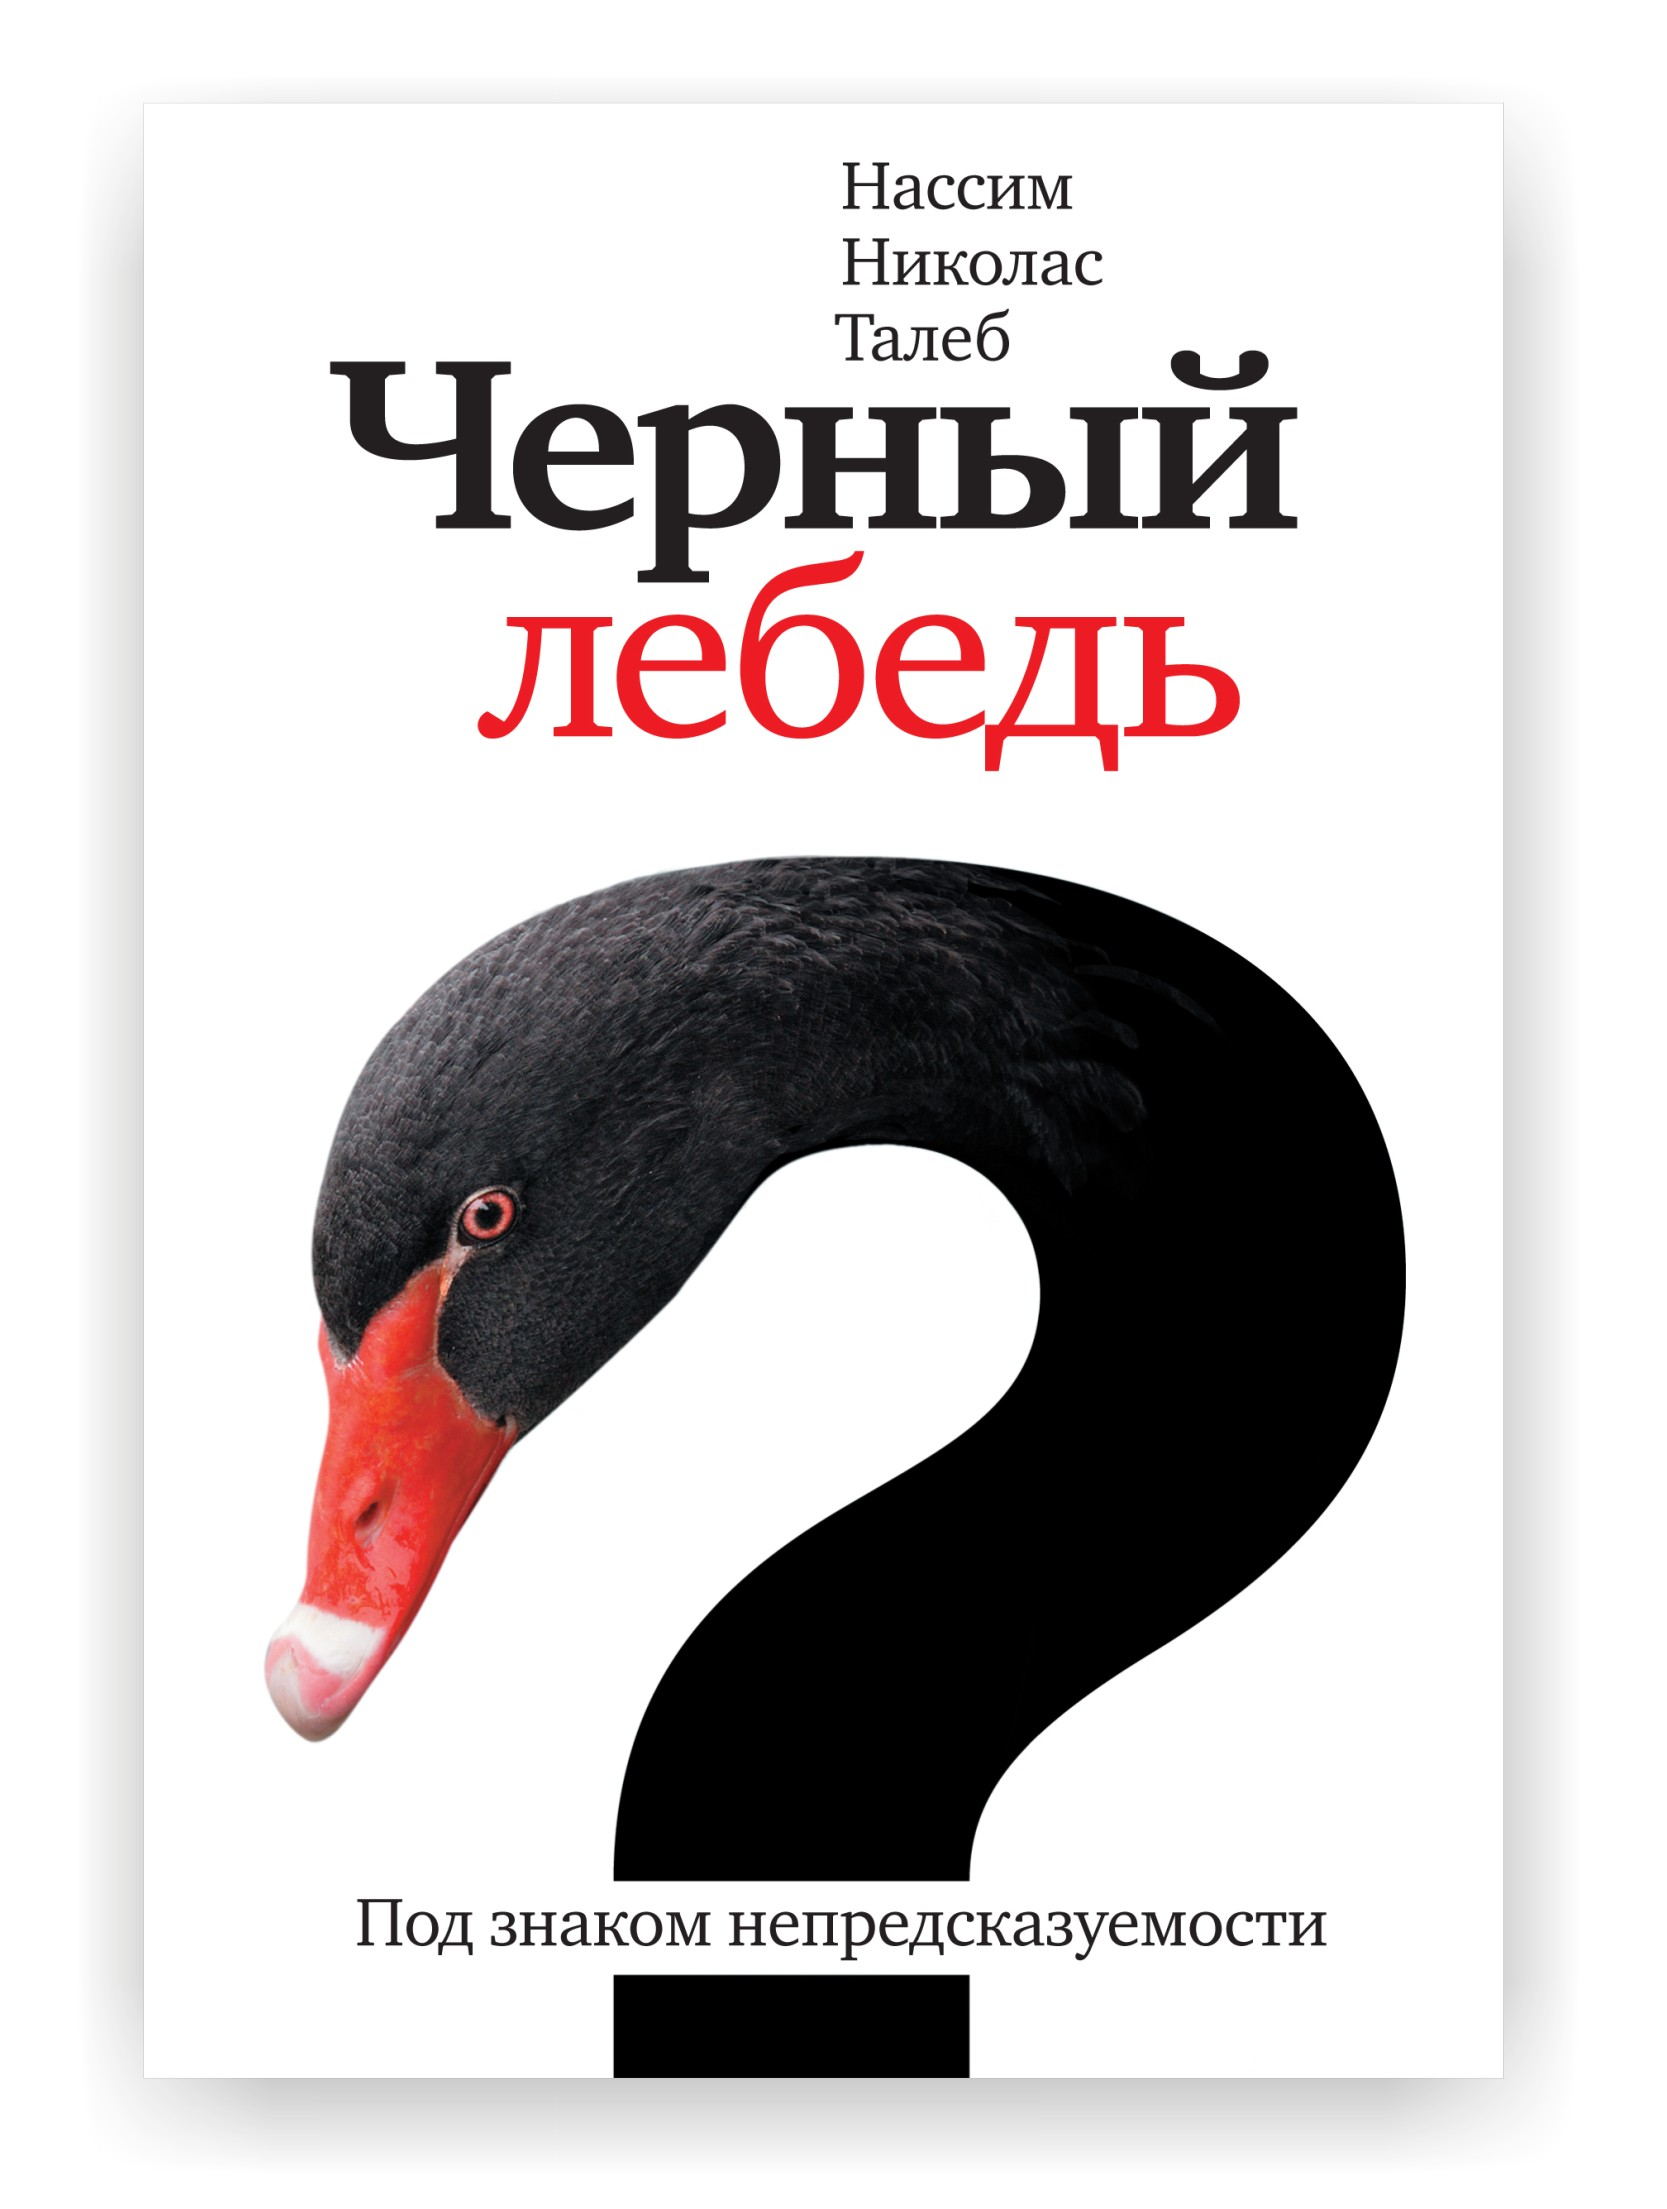
\includegraphics[width=1.0\textwidth]{black_swan.jpg}
    \caption{первое упоминание термина}
\end{figure}
\column{0.5\textwidth}
\begin{figure}
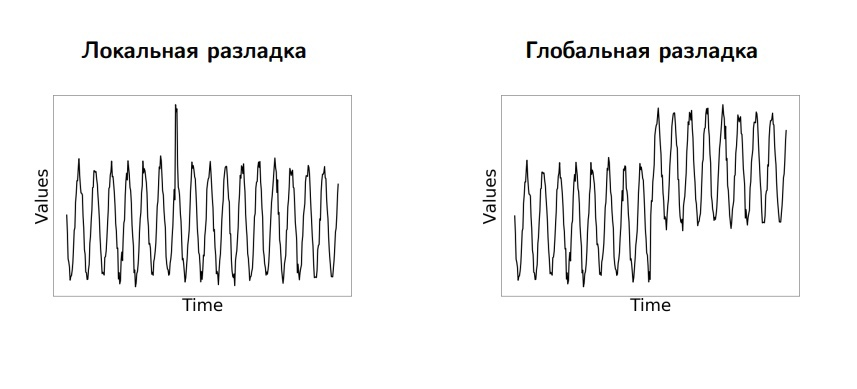
\includegraphics[width=1.0\textwidth]{razlad.jpg}
    \caption{случай временных рядов}
\end{figure}
\end{columns}

\end{frame}

\begin{frame}{Модель ResNet}

\begin{columns}[c]
\column{0.5\textwidth}
\par Изначально Neural ODE был разработан как альтернатива методу Residual Networks(ResNet), состоящих из последовательности скрытых слоёв, значения на каждом из которых подчинялись следующей формуле:
    \begin{equation} h_{k+1} = h_k + f(h_k, w_k)    \end{equation}
    \par --- где $h_k$ - вход k-го слоя для $k \in [1, K]$, $K$-число слоёв и f($h_k$, $w_k$) - функция, параметризованная по $w_k$ - динамический параметр, задающийся перед началом обучения модели.
\column{0.5\textwidth}
\begin{figure}
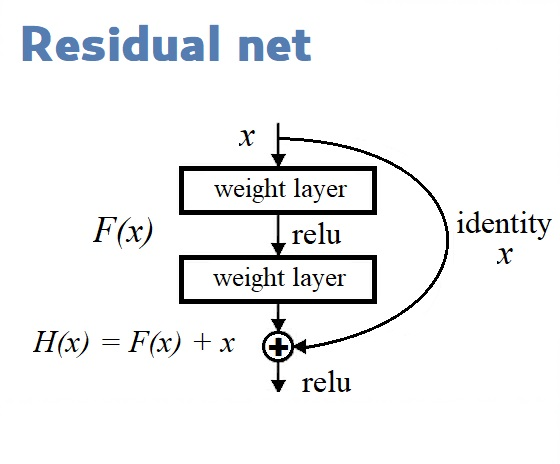
\includegraphics[width=1.0\textwidth]{resnet.jpg}
    \caption{схематичное описание работы}
\end{figure}
\end{columns}

\end{frame}

\begin{frame}{Модель Neural ODE}
\begin{equation} h_{t} = h_s + \int_s^t f(h_l, l; w) dl,    \end{equation}
    \par --- вычисление такого дифференциального уравнения является задачей для Neural ODE. В данной работе в качестве числа слоев берется число элементов во временном ряду.
    \begin{figure}
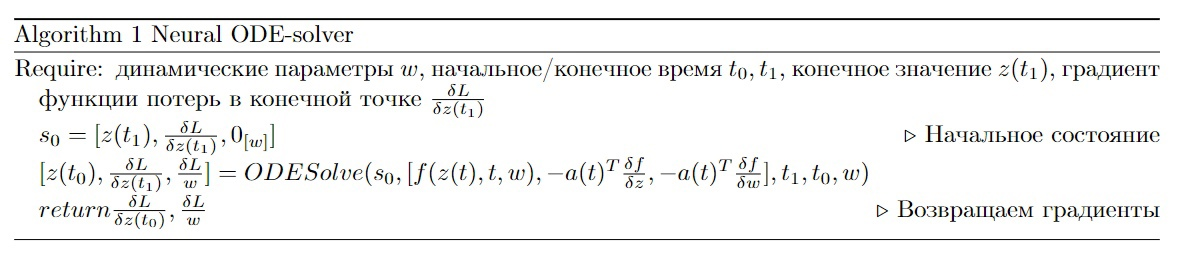
\includegraphics[width=1.0\textwidth]{algo.jpg}
    \caption{псевдокод Neural ODE}
\end{figure}
   \par Здесь ODESolve - это черный ящик, возвращающий решение ODE --- в качестве него предлагается использовать метод Рунге-Кутта, а L --- MSE~(mean squared error --- среднее квадратов отклонения элементов выборки от их оценок).

\end{frame}

\begin{frame}{Переход к Neural SDE}

\par Для учёта шума в наше дифференциальное уравнение следует добавить недетерменированную компоненту, диффузию. Получится следующее выражение, являющееся интегралом Стратоновича:
      \begin{equation} dX_t^w = h(t, X_t^w; w) dt + \sigma(X_t^w;w) dB_t     \end{equation}
      \par --- где $B_t=[B_t^1...B_t^K]$ - Винеровский процесс той же размерности, что и $X_t$, а $\sigma(X_t^w;w)$ - его матрица ковариаций в t-й момент времени
      \par Обобщим это выражение для модели ResNet:
      \begin{equation}  dh_t = f(h_t, t, w),    \end{equation}
      \par --- таким образом выражение (1) для (k+1)-го слоя изменится:
      \begin{equation} h_{k+1} = h_k + f(h_k, w_k) +  \sigma(X_k^w;w) B_k,    \end{equation}
      \par --- соответственно алгоритм остаётся тем же, что и для ODE с поправкой на вычисление матрицы ковариации элементов ряда.

\end{frame}


\begin{frame}{Пример выборки с неоднородной стохастической природой}

\begin{columns}[c]
\column{0.5\textwidth}
\begin{figure}
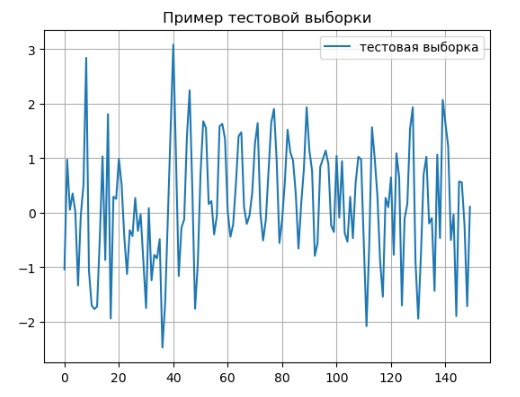
\includegraphics[width=1.0\textwidth]{sample_1.jpg}
    \caption{выборка}
\end{figure}
\column{0.5\textwidth}
\begin{figure}
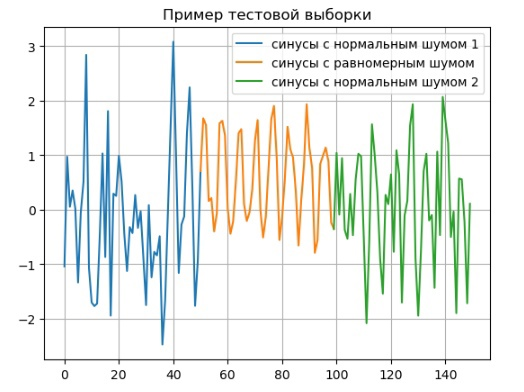
\includegraphics[width=1.0\textwidth]{sample_2.jpg}
    \caption{происхождение разных отрезков ряда}
    \end{figure}
\end{columns}

\end{frame}

\begin{frame}{Использование библиотеки torchSDE}


\begin{columns}[c]
\column{0.5\textwidth}
\begin{figure}
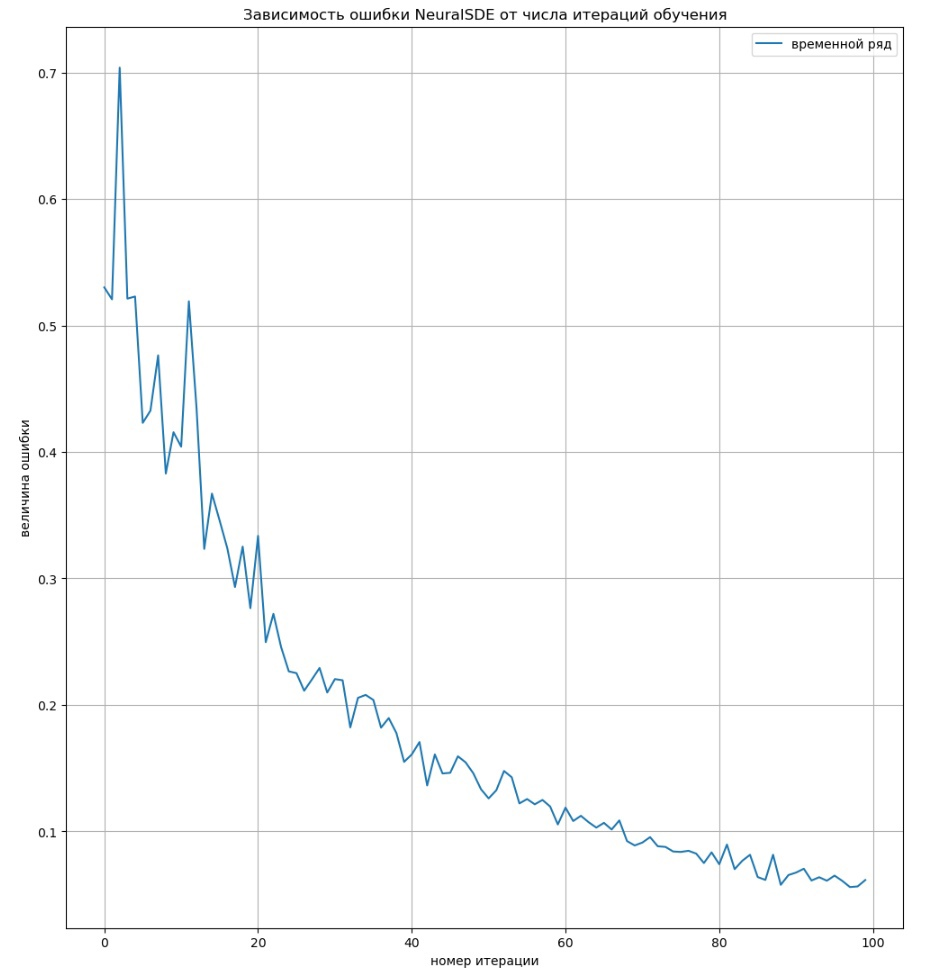
\includegraphics[width=1.0\textwidth]{loss.jpg}
    \caption{процесс обучения}
\end{figure}
\column{0.5\textwidth}
   \par Строится матрица Ганкеля, описывающая фазовые траектории процесса, размера (n+1) на w вида:
    \begin{equation}
 \begin{bmatrix}
   f_1 & f_2 & \cdots & f_{w} \\
   f_2 & f_3 & \cdots & f_{w + 1} \\
   \vdots  & \vdots  & \ddots & \vdots  \\
   f_{n + 1} & f_{n + 2} & \cdots & f_{n + w} 
 \end{bmatrix}
\end{equation}
\par --- где n - размер выборки, w - ширина окна.
\end{columns}

\end{frame}

\begin{frame}{Результаты поиска точек разладки}


\begin{figure}
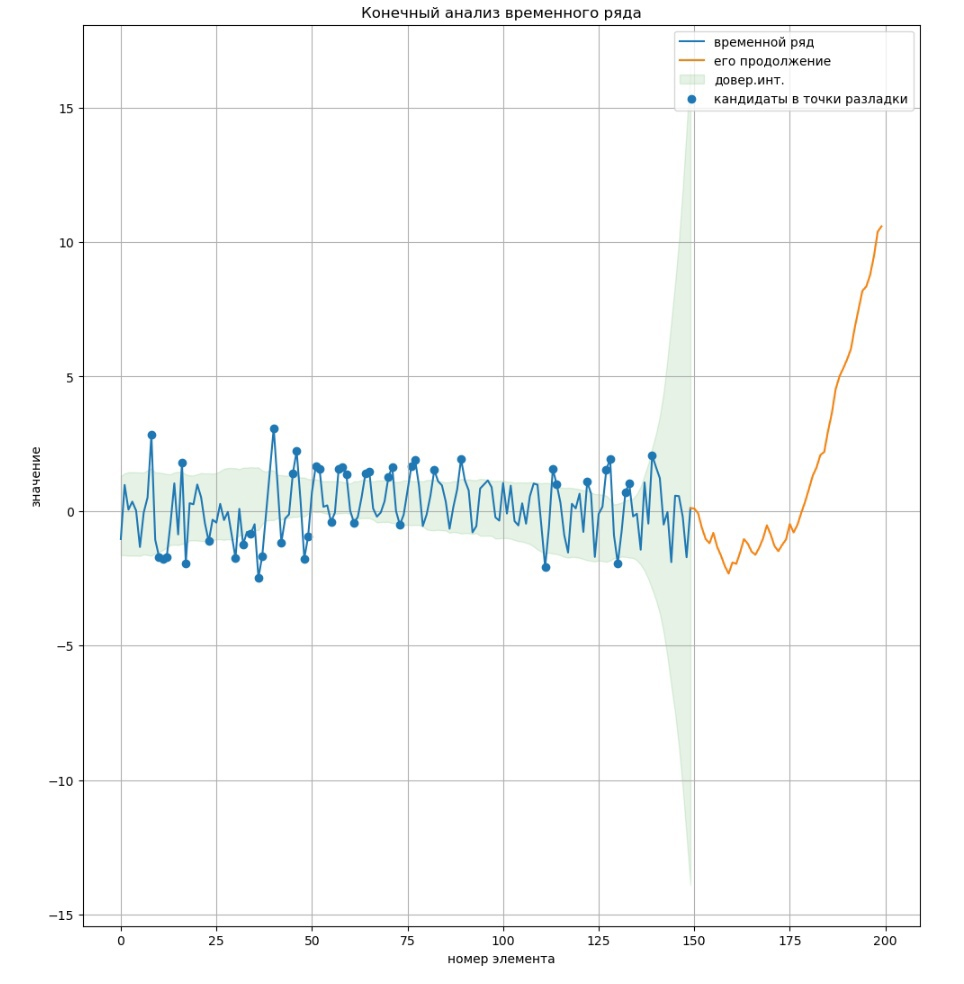
\includegraphics[height=0.6\textwidth]{result.jpg}
\caption{воссоздание их фаз.траекторий с помощью Neural SDE}
\end{figure}

\end{frame}

\begin{frame}{Источники}

[1] “Neural Ordinary Differential Equations Ricky” T. Q. Chen, Yulia Rubanova, Jesse Bettencourt, David Duvenaud \\

[2] “Neural SDE: Stabilizing Neural ODE Networks with Stochastic Noise” Xuanqing Liu, Tesi Xiao, Si Si, Qin Cao, Sanjiv Kumar, Cho-Jui Hsieh  \\

[3] “Riemannian Neural SDE: Learning Stochastic Representations on Manifolds” Sung Woo Park , Hyomin Kim , Kyungjae Lee , Junseok Kwon \\

[4] “Riemannian Diffusion Models” Chin-Wei Huang, Milad Aghajohari, Avishek Joey Bose, Prakash Panangaden, Aaron Courville \\

[5] Tian Qi Chen, Yulia Rubanova, Jesse Bettencourt, and David K Duvenaud. Neural ordinary differential equations. In Advances in Neural Information Processing Systems, pages 6572–6583, 2018. \\

[6] F.Yu. Yaushev, R. V. Isachenko, V. V. Strijov. Concordant models for latent space projections in forecasting, 2020. \\

\end{frame}


%----------------------------------------------------------------------------------------------------------
% \begin{frame}{Постановка задачи}
%
% \end{frame}
%----------------------------------------------------------------------------------------------------------
% \begin{frame}{Решение}
% \begin{columns}[c]
% \column{0.6\textwidth}
%     Столбец 1
% \column{0.4\textwidth}
%     Столбец 2
% \end{columns}
% \end{frame}
%----------------------------------------------------------------------------------------------------------
% \begin{frame}{Вычислительный эксперимент}
%
%  Что зритель видит на графике.
%
% \includegraphics[width=0.8\textwidth]{ErrorFunction}
%
% О чем говорит этот график.
%
% \end{frame}
%----------------------------------------------------------------------------------------------------------
% \begin{frame}{Заключение}
%     \begin{block}{Перечислите ваши результаты}
%     \begin{itemize}
%         \item предложен метод,
%         \item доказана теорема.
%     \end{itemize}
%     \end{block}
% \end{frame}
%----------------------------------------------------------------------------------------------------------

\end{document} 